\documentclass[a4paper,10pt]{article}

\usepackage[T1]{fontenc}
\usepackage[utf8]{inputenc}
\usepackage{graphicx}
\usepackage{xcolor}
\usepackage{fourier}
\usepackage{caption}
\usepackage{subcaption}
\usepackage{cprotect}
\usepackage{tgtermes}

\usepackage[
pdftitle={Computer Aided Diagnosis}, 
pdfauthor={Luc Nies, Tom van de Poll, Harmen Prins, Steven Reitsma \& Inez Wijnands, Radboud University Nijmegen},
colorlinks=true,linkcolor=blue,urlcolor=blue,citecolor=blue,bookmarks=true,bookmarksopenlevel=2]{hyperref}
\usepackage{amsmath,amssymb,amsthm,textcomp}
\usepackage{enumerate}
\usepackage{multicol}
\usepackage{tikz}

\usepackage{geometry}
\geometry{total={210mm,297mm},
left=25mm,right=25mm,%
bindingoffset=0mm, top=20mm,bottom=20mm}

\numberwithin{equation}{section} % Number equations within sections (i.e. 1.1 instead of 1)
\numberwithin{figure}{section} % Number figures within sections (i.e. 1.1 i/o 1)
\numberwithin{table}{section} % Number tables within sections (i.e. 1.1 i/of 1)

\linespread{1.35}

\newcommand{\linia}{\rule{\linewidth}{0.5pt}}

% my own titles
\makeatletter
\renewcommand{\maketitle}{
\begin{center}
\vspace{2ex}
{\huge \textsc{\@title}}
\vspace{1ex}
\\
\linia\\
\@author  \@date
\vspace{4ex}
\end{center}
}
\makeatother

% custom footers and headers
\usepackage{fancyhdr,lastpage}
\pagestyle{fancy}
\lhead{}
\chead{}
\rhead{}
\lfoot{Phase \textnumero{} 1}
\cfoot{}
\rfoot{Page \thepage\ /\ \pageref*{LastPage}}
\renewcommand{\headrulewidth}{0pt}
\renewcommand{\footrulewidth}{0pt}

% code listing settings
\usepackage{listings}
\lstset{
    language=Python,
    basicstyle=\ttfamily\small,
    aboveskip={0.9\baselineskip},
    belowskip={0.9\baselineskip},
    columns=fixed,
    extendedchars=true,
    breaklines=true,
    tabsize=4,
    prebreak=\raisebox{0ex}[0ex][0ex]{\ensuremath{\hookleftarrow}},
    frame=lines,
    showtabs=false,
    showspaces=false,
    showstringspaces=false,
    keywordstyle=\color[rgb]{0.1,0.126,0.941},
    commentstyle=\color[rgb]{0.133,0.545,0.133},
    stringstyle=\color[rgb]{0,0.5,0},
    numbers=left,
    numberstyle=\scriptsize\ttfamily,
    stepnumber=1,
    numbersep=10pt,
    captionpos=t,
    escapeinside={\%*}{*)}
}

%%%----------%%%----------%%%----------%%%----------%%%

\begin{document}

\title{Computer Aided Diagnosis \\\vspace{0.2cm} Lung segmentation}

\author{Luc Nies (s4136748), Tom van de Poll (s4106512), Harmen Prins (s4132297),\\ Steven Reitsma (s4132343) \& Inez Wijnands (s4149696)\\ Radboud University Nijmegen\\}

\date{11/05/2016}

\maketitle

\section{Problem description}

\section{Fully convolutional network}
Paper by Long et al \cite{long2015fully}

\section{Region growing in MeVisLab}
The biggest challenge with applying region growing in order to segment the lungs from and image is that in order to traditionally use region growing for segmentation, seed points need to be automatically selected inside the area that needs to be segmented. Since this is a difficult task, the descision is made to circumvent this problem by using region growing in a different way. The following algorithm is used for segmentation in MeVisLab:

\begin{itemize}
\item Threshold the image with threshold value 1000.
\item Apply region growing to the image, four times, with a corner pixel of the first slice as seed point.
\item Add the resulting four images to the thresholded image.
\item Threshold the resulting image with value 1000. An exmaple result can be seen in figure \ref{fig:reg-gro}.
\item Invert the resulting image. All that is left are the lungs and some other artifacts. An example can be seen in figure \ref{fig:lung-meuk}.
\item Do a connected components analysis on the resulting image, and select only the largest component from the image (the lungs).
\item Since there are still black holes in the lungs (veins), closing is applied to the image with a 10x10x1 spherical kernel. An example of the resulting segmentation mask can be seen in figure \ref{fig:lungs}.
\end{itemize}


This approach circumvents the need to find specific region growing seed points, since we take the same seed points for each image, namely the four corner pixels of the first slice. The results gathered with this method seem fairly promosing. More on the results of using this segmentation method is discussed in the results section


\section{Results}

\section{Conclusion}

\section{Contributions}

Luc Nies:

Steven Reitsma:

Harmen Prins:

Inez Wijnands:

Tom van de Poll: Contributed to the initial implementation of the fully convolutional network. Contributed to creating the MeVisLab segmentation method and responsible for troubleshooting this method. Implemented the method for looping the MeVisLab segmentation method over the data.\\

\section{appendix}
\begin{figure}[h]
	\centering
	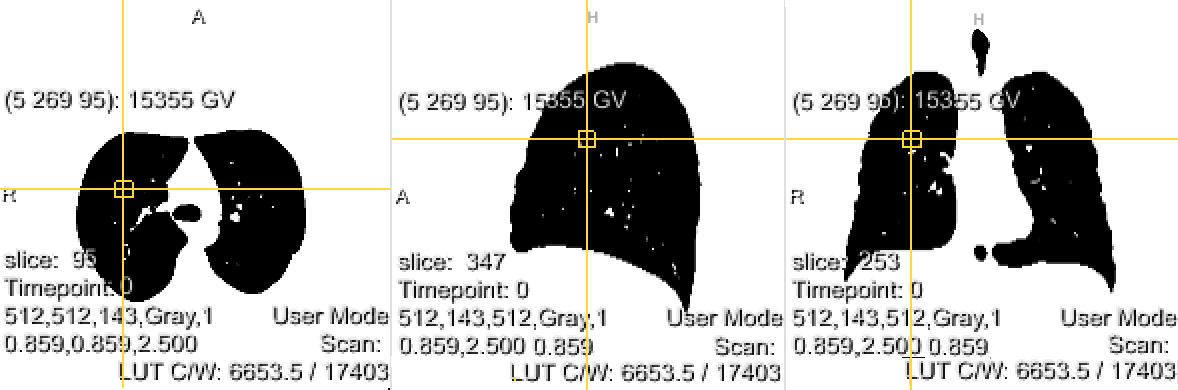
\includegraphics[scale=0.7]{regiongrowing}
    \caption{The thresholded image after region growing.}
    \label{fig:reg-gro}
\end{figure}


\begin{figure}[h]
    ~ %add desired spacing between images, e. g. ~, \quad, \qquad, \hfill etc. 
      %(or a blank line to force the subfigure onto a new line)
    \begin{subfigure}[b]{0.45\textwidth}
        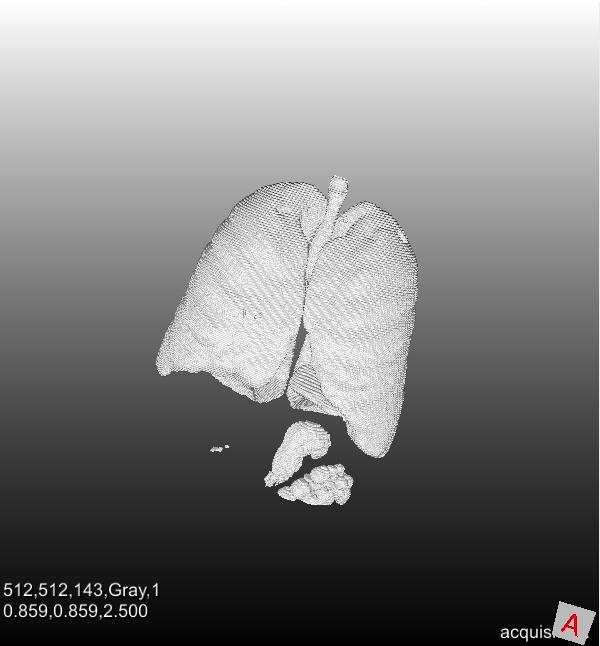
\includegraphics[width=\textwidth]{lungs_with_meuk}
        \caption{The image after the inversion step.}
        \label{fig:lung-meuk}
    \end{subfigure}
    ~ %add desired spacing between images, e. g. ~, \quad, \qquad, \hfill etc. 
    %(or a blank line to force the subfigure onto a new line)
    \begin{subfigure}[b]{0.45\textwidth}
        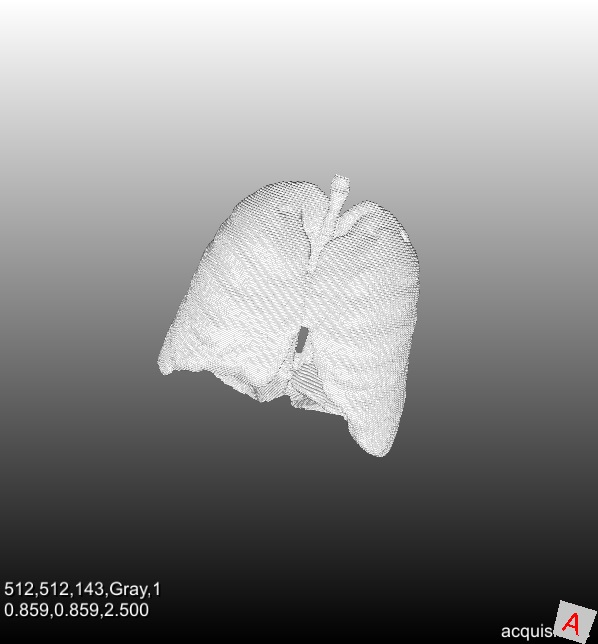
\includegraphics[width=\textwidth]{lungs_without_meuk}
        \caption{The result of the segmentation.}
        \label{fig:lungs}
    \end{subfigure}
    \caption{}\label{fig:lung-segmentation}
\end{figure}

\bibliographystyle{amsplain}
\bibliography{references}

\end{document}